\chapter{Исследовательский раздел}
В данном разделе представлены технические характеристики компьютера, используемого для тестирования, и результат работы программы.
 \section{Технические характеристики}

Ниже приведены технические характеристики устройства, на котором было проведено тестирование ПО:

\begin{itemize}
	\item операционная система: Windows 10 (64-разрядная);
	\item оперативная память: 32 GB;
	\item процессор: Intel(R) Core(TM) i7-7700K CPU @ 4.20GHz;
	\item количество ядер: 4;
	\item количество потоков: 8.
\end{itemize}

\section{Результат рыботы программы}
На рисунке \ref{results} представлены результаты работы программы для обработки 10 заявок каждая из которых содержит строку из 10000 слов состоящих из 1-10 букв.

\begin{figure}[h]
	\center{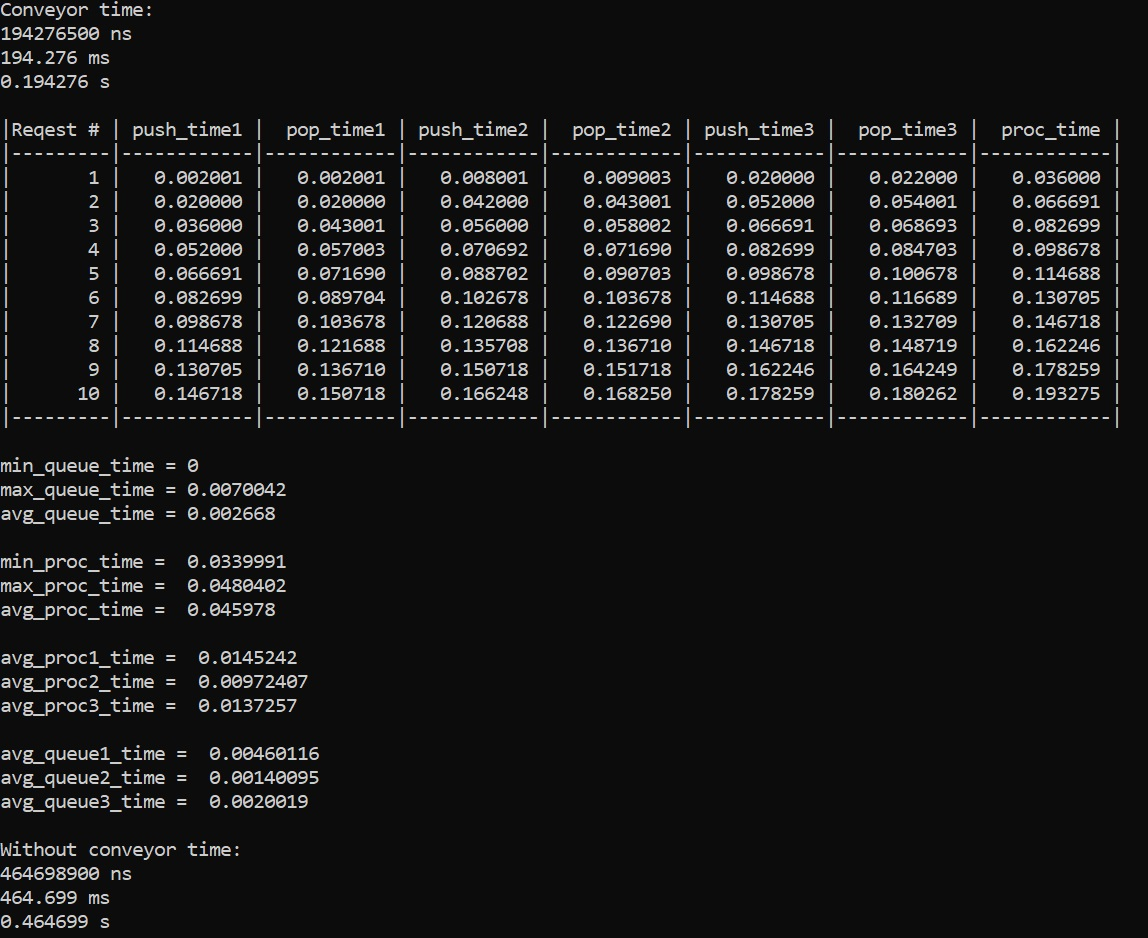
\includegraphics[width=1\linewidth]{inc/img/results}}
	\caption{Результат рыботы программы}
	\label{results}
\end{figure}

Из результатов следует, что больше все времени в среднем тратится на разбиение строки на слова, и меньше всего на поиск полиномов среди них. Время простоя в первой очереди --- наибольшее, а во второй --- наименьшее. Также, реализация с конвеером быстрее справилась с заявками, чем реализация с последовательной обработкой.

\newpage
\section{Вывод}
По итогу иследования выяснилось, что разработанный алгоритм работает верно, то-есть находит самый длинный полином в строке. Кроме этого был проведёно анализ и сделан вывод по логу программы.